%% A simple template for a scientific article using the Hagenberg setup
%% based on the standard LaTeX 'article' class
%%% äöüÄÖÜß  <-- no German umlauts here? Use a UTF-8 compatible editor!

%%% Magic comments for setting the correct parameters in compatible IDEs
% !TeX encoding = utf8
% !TeX program = pdflatex 
% !TeX spellcheck = en_US
% !BIB program = biber

\RequirePackage[utf8]{inputenc} % Remove when using lualatex or xelatex!
\RequirePackage{hgbpdfa}        % Creates a PDF/A-2b compliant document

\documentclass[english,smartquotes]{hgbarticle}
%\documentclass[english,twocolumn, smartquotes]{hgbarticle}
% Valid options in [..]: 
%    Main language: 'german' (default), 'english'
%    Turn on smart quote handling: 'smartquotes'
%    APA bibliography style: 'apa'
%    Typeset the text in two columns: 'twocolumn'
%%%-----------------------------------------------------------------------------

% for algorithm description
\usepackage{algorithm}
\usepackage{algpseudocodex}
% for algorithm description
\usepackage{lipsum}       % Create lorem ipsum dummy text (can be removed)
\usepackage{hyperref} % clickable www links
\hypersetup{
colorlinks=true,
linkcolor=blue,
urlcolor=magenta,
}
\flushbottom              % Add vertical space where necessary to fill the page
\graphicspath{{images/}}  % Location of images and graphics
\bibliography{references} % Biblatex bibliography file (references.bib)

% for unside down text
\usepackage[framemethod=tikz]{mdframed}
\newtheorem{question}{Puzzle}
\mdfdefinestyle{que}{
  linecolor=cyan,
  backgroundcolor=cyan!20,
}
\surroundwithmdframed[style=que]{question}
\newtheorem{answer}{}
\mdfdefinestyle{ans}{
  linecolor=cyan,
  backgroundcolor=cyan!20
}
\surroundwithmdframed[style=ans]{answer}
\usepackage{environ}
\NewEnviron{rotanswer}{%
  \begin{tikzpicture}
  \node[rotate=180,inner sep=0pt] {\parbox{\linewidth}{%
  \begin{answer}
  \BODY
  \end{answer}}};
\end{tikzpicture}%
}
% for unside down text https://tex.stackexchange.com/a/161886/64425
% for simple color box
\usepackage[most]{tcolorbox}
% for simple color box
% for simple arrays
% https://tex.stackexchange.com/a/31346/64425
\usepackage{tikz}
\usetikzlibrary{calc}
% for simple arrays
% for captions, but not floating
% https://tex.stackexchange.com/a/7212/64425
% \usepackage{caption}

\DeclareCaptionType{mytype}[Fig][List of mytype]
\newenvironment{arrangement}{\captionsetup{type=mytype}}{}


% for captions, but not floating
%%%-----------------------------------------------------------------------------
\begin{document}
%%%-----------------------------------------------------------------------------

\author{
	Kedar Mhaswade\\ 
	\email{kedar.mhaswade@gmail.com}
}
\title{A Social Media Combinatorial Problem}
\date{}

%%%-----------------------------------------------------------------------------
\maketitle
%%%-----------------------------------------------------------------------------
%\listofmytypes % captioning

\begin{abstract}\noindent
This article discusses an algorithmic approach and a computer program based on it to solve an elementary combinatorial problem that is popular on social media. Our intended audience is high school students (and laypeople) with an aptitude for abstract thinking and an interest in problem-solving. The algorithm presented here is correct but inefficient. However, it sheds light on a well-known problem in theoretical computer science.
\end{abstract}

%%%-----------------------------------------------------------------------------

\section{Introduction}

Consider a puzzle popular on social media\footnote{I first heard it from \href{https://sunilsingh-42118.medium.com/}{Sunil Singh}, a mathematics educator}:

\begin{question}
\label{puzzle1}
How can you make $24$ using the numbers $1, 3, 4,$ and $6$ exactly once each, and the four arithmetic operations ($+, -, \times, \div$) any number of times\footnote{Using a number by concatenating two or more numbers (e.g., $13$) is not allowed}?
\end{question}

A ready-made answer is probably just an Internet search\footnote{Or a chat with your favorite Large Language or Reasoning Model or agentic AI} away. Just for fun, however, one should find such an arithmetic expression without searching it on the Web. Try it before you read further. Don't worry, the author took quite some time to find it. If you don't find an answer and are restless, skip to the end.

\subsection{Initial Impressions}
This puzzle is surprisingly challenging, especially if one is not well-versed in solving such puzzles. We take arithmetic for granted, but the four basic operations combine with four small numbers to render it tantalizingly difficult. This is so even if you could solve it.

In our attempts, we may start with heuristics: If we can make an \textit{expression} using 1, 3, and 4 that evaluates to 4, then we can make 24 by multiplying it by 6. But now we have a different puzzle that is just as tricky.

We may try parenthesizing parts of shorter expressions and combining their results (e.g. $((6+4)-1)\times3 = 27$). After toiling for a while we might \textit{luckily} find the magic expression.

But we may not. What if no such expression exists? Can we tell if one exists at all? If more than one solution exists, can we find them all? Can we even tell if we have examined \textit{all} expressions possible?

We keep \textit{feeling} inadequate as we continue searching \dots
\section{An Algorithmic Approach to Searching}
As we keep searching, we may feel frustrated. After all, what we repetitively do is make expressions of four small numbers and four familiar arithmetic signs and evaluate them. It gets quite mechanical and hence boring after a short while. But we tend not to give up for a perceived shame grips us. After all, we have been seeing such numbers and signs since first grade!

Even if we solve the puzzle, we wonder if we weren't lucky. If we are about to abandon\footnote{Indeed, a friend, after trying for a while, hesitantly asked the author, ``Do you know if a solution exists?''} the search and declare that no solution exists, we seem to lack the confidence that we have indeed examined every expression. 

Most of all, we feel the need for assistance from a machine that accepts (or, better yet, constructs) expressions and evaluates them correctly and, well, mechanically. It's a solace that just such an accomplice exists: A computer! 

A computer is astoundingly fast at performing known calculations precisely and, at the same time, naturally incapable of possessing intelligence\footnote{AI techniques claim to rectify that limitation} or originality in devising \textit{abstractions}, the basis of computing. Alan Perlis once said \cite{Perlis1984} that, like a few other things, a computer, by definition, is \textit{explicitly programmed}. 

Typically, a computer depends on us to tell it something (worthwhile) to do. And it needs precise, formal instructions. Or, more factually, we have got to believe that it follows our instructions precisely. If the outcome of those instructions is different from what we expect, then we must doubt our instructions and it is up to us to modify them. We must not doubt if the computer followed them dutifully and precisely. 
% To our dismay or our pleasant surprise, ``AI-powered'' computers have started showing signs of a startling but \textit{disembodied} intelligence, but we will save that topic for later.  

Clear instructions are called an \emph{algorithm}. Clearly, we need an algorithm to solve every problem we delegate to the computer. Perhaps surprisingly, however, the idea of an algorithm is independent of a physical computer. According to Donald Knuth \cite{Knuth1997}, Euclid described the first ``computer algorithm'', known as Euclid's GCD algorithm, more than 2200 years before the advent of a digital computer!

So, how do we fit this puzzle within the confines of the strict formalism that a computer demands? If only we could construct every expression \dots

\subsection{Some Formal Background}
To develop a perspective, we need to precisely define \textit{expression}, \textit{operator}, and \textit{operand}. An operator has a symbol and describes an operation on several operands which are just numbers in our case. Every operation \textit{takes} some operands and \textit{produces} a result (or results) that is, in many ways, like its operands--again, numbers in our case. Depending upon how many operands the operation takes, an operator can be classified \textit{unary} (takes one operand), \textit{binary} (takes two operands), etc. This property of an operator is called its \textit{arity}. Operators can also be \emph{commutative} or \emph{non-commutative}. Results of commutative binary operators do not depend on the \emph{order} of their operands: $a+b=b+a$, whereas those of non-commutative binary operators do: $a\div b \ne b\div a$ 

We learn in grade school that unary operator symbols are written either before the numbers (e.g. $\sqrt 8$ to denote the square root of 8) or after the numbers (e.g. $3!$ to denote the factorial of 3), whereas the binary operator symbols are written between them ($2 + 3 = 5$). For binary operators, such an expression is called an \emph{infix} expression.

The four basic arithmetic operations--addition, subtraction, multiplication, and division-- are all binary. They take two numbers and produce a number. That helps us combine them sequentially to form expressions. Each expression can be \textit{evaluated} to produce a value which is a number in our case.

Combining operations in expressions such as $2+3+8+7$ achieve brevity\footnote{Imagine the plight of reading $2+3; 5+8; 13+7$ instead} which aids comprehension. However, ambiguity arises when different operators appear in the same expression: $1+2\times 3$ because we don't know whether to add first and then multiply (producing 9) or vice versa (producing 7). To address the ambiguity, we could have made a rule: \textit{Do the operations in the order of their appearance}.  

Instead, we use parentheses to disambiguate: $(1+2)\times 3$ evaluates to 9 and $1+(2\times 3)$ to 7. If we do not want to introduce parentheses, however, we need to define \textit{precedence} of operators. This is where the mnemonics like ``BODMAS'' originate.  Infix notation is a rules-heavy way to denote and evaluate expressions. But is that the only way?

\subsection{Postfix Expressions and the Stack}
As students, we should develop the habit of \emph{meaningfully challenging the status quo}. History of mathematics and other sciences teaches us about people who dared to explore and we learn a great deal about trailblazing from them.

The Polish logician Jan Łukasiewicz\footnote{Pronounced \textit{yahn woo-ka-shay-vitch}} proposed a different idea for the notation\cite{Hamblin1962}: \textbf{Place the symbol after (or before) the operands}. We call such an expression a \emph{postfix}\footnote{It's also called the \emph{Reverse Polish notation}} (or \emph{prefix}) expression. Thus, the postfix expression corresponding to the first expression above is $1\;2 + 3\times$ and that to the second is $1\;2\;3\times +$. 

To evaluate expressions, we propose the idea of a \emph{stack}. A stack is an abstract structure that resembles a stack of dishes we often see at restaurants. If we only allow adding and removing a dish to and from the top of the stack then it makes a dish added last to be removed first. This view makes stack a linear queue whose elements are added and removed only from one of its two ends--the top\footnote{A stack is therefore called a LIFO--Last In First Out--queue}. 

Two operations on a stack are essential: 1) \texttt{push element}, which pushes the given element on the stack, and 2) \texttt{pop} which simply removes the element at the top of the stack, and returns its value. Doing the \texttt{push} operation once increments the \emph{size} of the stack whereas doing the \texttt{pop} operation once decrements it.

If you have never encountered a stack before, you may not be impressed with the immense power its simplicity offers to \emph{model} in many practical situations. But that is the usefulness of abstractions: It doesn't matter to the stack what it is employed to store (dishes, objects, or numbers). It provides a structure to store it and the two essential operations: \texttt{push} and \texttt{pop} defined above. Optionally, we may want to know if the stack is empty (in which case we can't \texttt{pop} an element) or the stack is full (which can happen in practice where resources are limited and we can't \texttt{push} an element).

Perhaps you are thinking of postfix expressions as an unnecessary digression. You may be wondering why a postfix expression like: $1\;2\;3\times +$ is more convenient than the corresponding infix expression: $1+(2\times 3)$.

And one might even successfully argue that infix expressions are easier to read. But isn't readability a question of getting used to? Had we been reading postfix expressions since grade school, we might have become more comfortable with them. Is there another benefit? 

It turns out that postfix expressions need no operator precedence rules, and, as a result, they do not need parenthesizing expressions to enforce precedence. A given postfix expression can be evaluated \emph{mechanically} (with the help of the stack)! This bonus becomes apparent when we study the \emph{algorithmic} nature of evaluating postfix expressions. 

We start with a postfix expression. For the sake of our algorithm, we read it a \textit{token} at a time. A token is either an operand or an operator. Our operators are all binary. However, the scheme can be easily extended to other operators (e.g. unary). We use the stack only to store operands and results of operations. Thus, ours is a stack of numbers. Here is our Algorithm[\ref{alg1}].
\begin{algorithm}
\caption{Evaluate any postfix expression with binary operators}
\label{alg1}
\begin{algorithmic}[1]
  \State $S \gets \Call{Stack.New}{}$
  \State $T \gets [t_1, t_2, \dots,t_n]$
	\While{T has tokens} \Comment{Start scanning the expression from left}
	  \State $t \gets$\Call{T.next}{}
		\If{$t$ is an operand}
			\State \Call {S.push}{t} \Comment{\textcolor{red}{Return Error if the stack is full}}
		\ElsIf{$t$ is an operator} \Comment{Write defensive program}
			\State $o2 \gets$ \Call {S.pop}{} \Comment{Pop \textit{two} operands}
			\State $o1 \gets$ \Call {S.pop}{} \Comment{Order matters; pop second operand first}
			\\
			\Comment{\textcolor{red}{Return Error if the stack doesn't have enough operands to pop}}
			\State $r \gets$ \Call {op}{od1, od2} \Comment{e.g. 2 + 3 and $r \gets 5$}
			\State \Call {S.push}{r}\Comment{\textcolor{red}{Return Error if the stack is full}}
		\Else 
		  \State \textcolor{red}{return Error} \Comment{Impossible? An invalid token}
		\EndIf
	\EndWhile
	\If{\Call{S.empty}{}?}
	  \State \textcolor{red}{return Error} \Comment{S must have the result}
	\Else 
	  \State return \Call{S.pop}{} \Comment{A valid expression evaluates to this value}
	\EndIf
\end{algorithmic}
\end{algorithm}

\subsection{A Helpful Insight?}
Infix and postfix (or prefix), after all, are just notations. And it so happens that one can deterministically translate a valid infix expression into postfix and vice versa. 
However, removing the need for parentheses and providing a mechanical way of evaluating are strengths of the postfix expression which the author used to address our puzzle \ref{puzzle1}. Let's list the helpful facts that we know so far. They may sound disparate at the moment, but they might align themselves in a coherent whole later:
\begin{tcolorbox}
[
colback=yellow!20,
colframe=cyan,
sharp corners,
boxrule=0.5pt,
]
We want to employ a (preferably systematic) method to \emph{assuredly} examine all expressions made of exactly four numbers ($1, 3, 4, 6$) and required (binary) arithmetic operators ($+, -, \times, \div$). The emphasis is on not missing any valid expression. \\

Can postfix notation help? \\

Since there are four operands and each \emph{binary} operator takes two operands and produces a result (which may then pair up with the next operand), we must have exactly three binary operators in an expression with seven tokens.
\end{tcolorbox}

We have four operands that can appear in any order in a postfix expression. Since we must have exactly three binary operators to operate on them, there are seven places each of which is occupied either by an operator or an operand. 

Here is a possible arrangement:

\begin{arrangement}
\vspace{2mm}
\centering
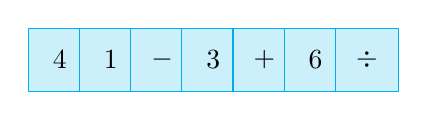
\begin{tikzpicture}
  \coordinate (s) at (0,0);
  \foreach \token in {4,1,-,3,+,6,\div}{
    \node[fill=cyan!20, minimum size=8mm, draw=cyan, rectangle] at (s) {$\token$};
    \coordinate (s) at ($(s) + (0.65,0)$);
  }
\end{tikzpicture}
\label{goodperm1}
\captionof{mytype}{A Valid Arrangement}
\end{arrangement}

Luckily, this is a valid postfix expression that evaluates to 1. We can trace the run of our algorithm [\ref{alg1}] on this expression to confirm the result.

Here is another possible arrangement:

\begin{arrangement}
\vspace{2mm}
\centering
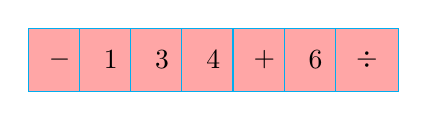
\begin{tikzpicture}
  \coordinate (s) at (0,0);
  \foreach \token in {-,1,3,4,+,6,\div}{
    \node[fill=red!35, minimum size=8mm, draw=cyan, rectangle] at (s) {$\token$};
    \coordinate (s) at ($(s) + (0.65,0)$);
  }
\end{tikzpicture}
\captionof{mytype}{A Valid Arrangement, but Invalid Postfix Expression}
\label{badperm1}
\end{arrangement}

We are unlucky in this case because this arrangement is not a valid postfix expression; it does not evaluate to any value. Expectedly, our algorithm [\ref{alg1}] returns an error in this case. But a computer doesn't care and perhaps neither should we, because we can ignore this arrangement as a ``non-expression'' and examine the next one. It would be nice to know a priori that such an expression is invalid (without actually evaluating it with our algorithm [\ref{alg1}]), but that is not necessary. The human mind may \emph{immediately} discard all the expressions like [\ref{badperm1}] that begin with an operator (because there is nothing to operate it on). But even an inefficient computer algorithm can sometimes beat that ingenuity with the shear speed of (possibly needless) calculation. 

This does not mean we write sloppy algorithms. We should always look for opportunities to optimize algorithms once their correctness is established. However, the nature of some problems makes it (very) difficult for us to devise efficient algorithms to solve them. Our problem shows symptoms of such a problem \dots

\subsection{The Algorithm}
Perhaps we now feel closer to describing a foolproof\footnote{Being foolproof is required because a computer is going to carry it out}, if inefficient, method of solving our puzzle to the computer. Our search has got to be exhaustive; \textbf{we must not miss any (valid) arrangement of four operands and three binary operators} but it is acceptable if some arrangement leads to an invalid expression. We evaluate each expression. If an expression evaluates to our target number (24), we have succeeded. If there is no such expression, the puzzle is unsolvable. An algorithm seems to emerge. We just need to describe the process precisely \dots

We are given a set of operands, but where they appear in the seven locations (their \emph{order}) matters. This is an archetypal situation leading us to a fascinating area of mathematics called Combinatorics. Specifically, we can arrange $k$ objects in $n$ locations\footnote{Each such arrangement is called a \emph{Permutation}} in ${}_{n}P_{k} = \frac{n!}{(n-k)!}$ ways. In our case, the number of such \emph{ordered arrangements} of four operands in seven locations is $\frac{7!}{3!}=7\times 6\times 5\times 4 = 840$. Here are some of the arrangements:

\begin{arrangement}
\vspace{2mm}
\centering
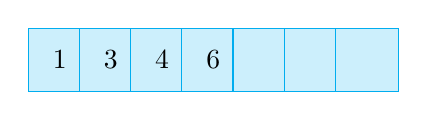
\begin{tikzpicture}
  \coordinate (s) at (0,0);
  \foreach \token in {1,3,4,6,\,,\,,\,}{
    \node[fill=cyan!20, minimum size=8mm, draw=cyan, rectangle] at (s) {$\token$};
    \coordinate (s) at ($(s) + (0.65,0)$);
  }
\end{tikzpicture}
\\
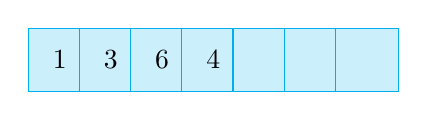
\begin{tikzpicture}
  \coordinate (s) at (0,0);
  \foreach \token in {1,3,6,4,\,,\,,\,}{
    \node[fill=cyan!20, minimum size=8mm, draw=cyan, rectangle] at (s) {$\token$};
    \coordinate (s) at ($(s) + (0.65,0)$);
  }
\end{tikzpicture}
\\
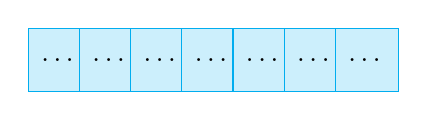
\begin{tikzpicture}
  \coordinate (s) at (0,0);
  \foreach \token in {\dots,\dots,\dots,\dots,\dots,\dots,\dots}{
    \node[fill=cyan!20, minimum size=8mm, draw=cyan, rectangle] at (s) {$\token$};
    \coordinate (s) at ($(s) + (0.65,0)$);
  }
\end{tikzpicture}
\\
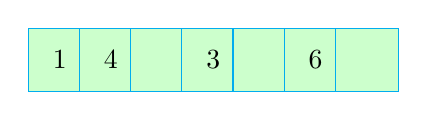
\begin{tikzpicture}
  \coordinate (s) at (0,0);
  \foreach \token in {1,4,\,,3,\,,6,\,}{
    \node[fill=green!20, minimum size=8mm, draw=cyan, rectangle] at (s) {$\token$};
    \coordinate (s) at ($(s) + (0.65,0)$);
  }
\end{tikzpicture}
\\
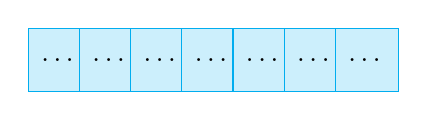
\begin{tikzpicture}
  \coordinate (s) at (0,0);
  \foreach \token in {\dots,\dots,\dots,\dots,\dots,\dots,\dots}{
    \node[fill=cyan!20, minimum size=8mm, draw=cyan, rectangle] at (s) {$\token$};
    \coordinate (s) at ($(s) + (0.65,0)$);
  }
\end{tikzpicture}
\\
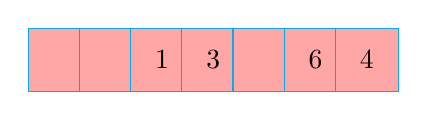
\begin{tikzpicture}
  \coordinate (s) at (0,0);
  \foreach \token in {\,,\,,1,3,\,,6, 4}{
    \node[fill=red!35, minimum size=8mm, draw=cyan, rectangle] at (s) {$\token$};
    \coordinate (s) at ($(s) + (0.65,0)$);
  }
\end{tikzpicture}
\\
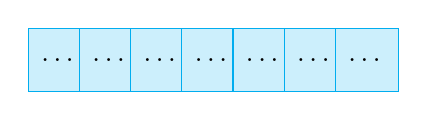
\begin{tikzpicture}
  \coordinate (s) at (0,0);
  \foreach \token in {\dots,\dots,\dots,\dots,\dots,\dots,\dots}{
    \node[fill=cyan!20, minimum size=8mm, draw=cyan, rectangle] at (s) {$\token$};
    \coordinate (s) at ($(s) + (0.65,0)$);
  }
\end{tikzpicture}
\\
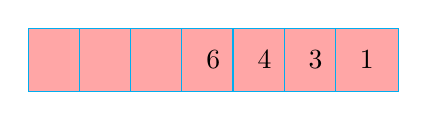
\begin{tikzpicture}
  \coordinate (s) at (0,0);
  \foreach \token in {\,,\,,\,,6,4,3,1}{
    \node[fill=red!35, minimum size=8mm, draw=cyan, rectangle] at (s) {$\token$};
    \coordinate (s) at ($(s) + (0.65,0)$);
  }
\end{tikzpicture}
\captionof{mytype}{All Permutations of Four in Seven}
\label{allperms}
\end{arrangement}

These are \emph{all} the possible ways in which we can arrange members of the set of operands $\{1,3, 4, 6\}$ in seven places, and there are exactly 840 such arrangements. Some arrangements will invariably lead to invalid postfix expressions (e.g. the permutations in red in Fig [\ref{allperms}]) after we place the operator symbols in the remaining places. 

How do we place operator symbols? Well, we have three places and we want to place three operators in them. However, this time repetition is allowed because we can choose the same operator more than once. Such arrangements where members of an $n$-set are placed in $k$ places (where choosing a set member more than once is allowed) are called $k$-tuples \cite{ktuples} of the $n$-set. The number of $k$-tuples is $n^{k}$. In our case $k=3, n=4, n^k=64$. We have 64 3-tuples of 4 operators to consider.

Let's demonstrate the placement of all operator 3-tuples with one arrangement of operands, $[$1,4,\textvisiblespace,3,\textvisiblespace,6,\textvisiblespace$]$, (shown in green) from Figure \ref{allperms}.

\begin{arrangement}
  \vspace{2mm}
  \centering
  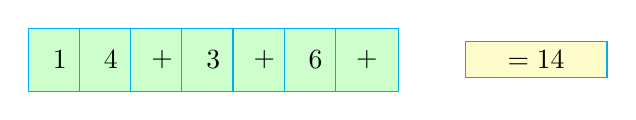
\begin{tikzpicture}
    \coordinate (s) at (0,0);
    \foreach \token in {1,4,+,3,+,6,+}{
      \node[fill=green!20, minimum size=8mm, draw=cyan, rectangle] at (s) {$\token$};
      \coordinate (s) at ($(s) + (0.65,0)$);
    }
    \coordinate (s) at ($(s) + (1.5,0)$);
    \node[fill=yellow!20, minimum width=18mm, draw=cyan, rectangle] at (s) {$=14$};
  \end{tikzpicture}
  \\
  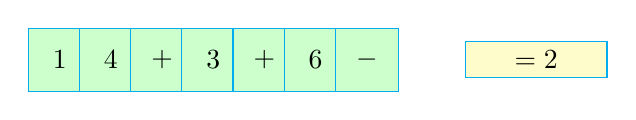
\begin{tikzpicture}
    \coordinate (s) at (0,0);
    \foreach \token in {1,4,+,3,+,6,-}{
      \node[fill=green!20, minimum size=8mm, draw=cyan, rectangle] at (s) {$\token$};
      \coordinate (s) at ($(s) + (0.65,0)$);
    }
    \coordinate (s) at ($(s) + (1.5,0)$);
    \node[fill=yellow!20, minimum width=18mm, draw=cyan, rectangle] at (s) {$=2$};
  \end{tikzpicture}
  \\
  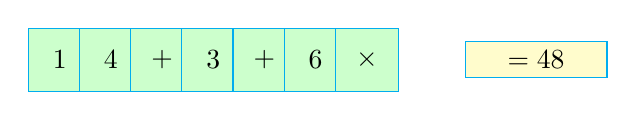
\begin{tikzpicture}
    \coordinate (s) at (0,0);
    \foreach \token in {1,4,+,3,+,6,\times}{
      \node[fill=green!20, minimum size=8mm, draw=cyan, rectangle] at (s) {$\token$};
      \coordinate (s) at ($(s) + (0.65,0)$);
    }
    \coordinate (s) at ($(s) + (1.5,0)$);
    \node[fill=yellow!20, minimum width=18mm, draw=cyan, rectangle] at (s) {$=48$};
  \end{tikzpicture}
  \\
  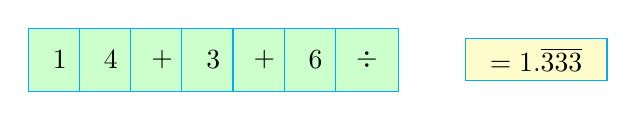
\begin{tikzpicture}
    \coordinate (s) at (0,0);
    \foreach \token in {1,4,+,3,+,6,\div}{
      \node[fill=green!20, minimum size=8mm, draw=cyan, rectangle] at (s) {$\token$};
      \coordinate (s) at ($(s) + (0.65,0)$);
    }
    \coordinate (s) at ($(s) + (1.5,0)$);
    \node[fill=yellow!20, minimum width=18mm, draw=cyan, rectangle] at (s) {$=1.\overline{333}$};
  \end{tikzpicture}
  \\
  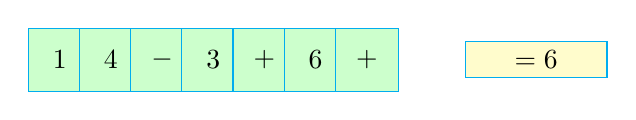
\begin{tikzpicture}
    \coordinate (s) at (0,0);
    \foreach \token in {1,4,-,3,+,6,+}{
      \node[fill=green!20, minimum size=8mm, draw=cyan, rectangle] at (s) {$\token$};
      \coordinate (s) at ($(s) + (0.65,0)$);
    }
    \coordinate (s) at ($(s) + (1.5,0)$);
    \node[fill=yellow!20, minimum width=18mm, draw=cyan, rectangle] at (s) {$=6$};
  \end{tikzpicture}
  \\
  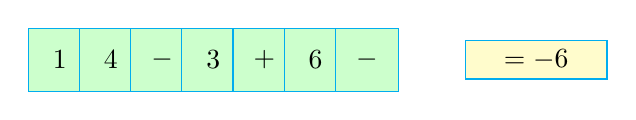
\begin{tikzpicture}
    \coordinate (s) at (0,0);
    \foreach \token in {1,4,-,3,+,6,-}{
      \node[fill=green!20, minimum size=8mm, draw=cyan, rectangle] at (s) {$\token$};
      \coordinate (s) at ($(s) + (0.65,0)$);
    }
    \coordinate (s) at ($(s) + (1.5,0)$);
    \node[fill=yellow!20, minimum width=18mm, draw=cyan, rectangle] at (s) {$=-6$};
  \end{tikzpicture}
  \\
  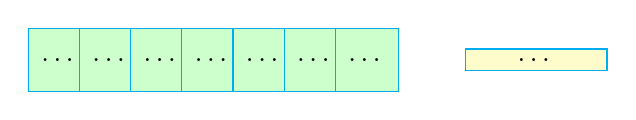
\begin{tikzpicture}
    \coordinate (s) at (0,0);
    \foreach \token in {\dots,\dots,\dots,\dots,\dots,\dots,\dots}{
      \node[fill=green!20, minimum size=8mm, draw=cyan, rectangle] at (s) {$\token$};
      \coordinate (s) at ($(s) + (0.65,0)$);
    }
    \coordinate (s) at ($(s) + (1.5,0)$);
    \node[fill=yellow!20, minimum width=18mm, draw=cyan, rectangle] at (s) {$\dots$};
  \end{tikzpicture}
  \\
  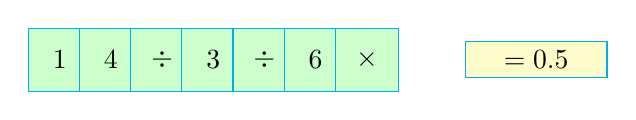
\begin{tikzpicture}
    \coordinate (s) at (0,0);
    \foreach \token in {1,4,\div,3,\div,6,\times}{
      \node[fill=green!20, minimum size=8mm, draw=cyan, rectangle] at (s) {$\token$};
      \coordinate (s) at ($(s) + (0.65,0)$);
    }
    \coordinate (s) at ($(s) + (1.5,0)$);
    \node[fill=yellow!20, minimum width=18mm, draw=cyan, rectangle] at (s) {$=0.5$};
  \end{tikzpicture}
  \\
  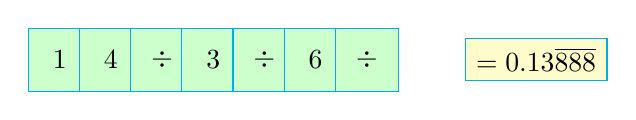
\begin{tikzpicture}
    \coordinate (s) at (0,0);
    \foreach \token in {1,4,\div,3,\div,6,\div}{
      \node[fill=green!20, minimum size=8mm, draw=cyan, rectangle] at (s) {$\token$};
      \coordinate (s) at ($(s) + (0.65,0)$);
    }
    \coordinate (s) at ($(s) + (1.5,0)$);
    \node[fill=yellow!20, minimum width=18mm, draw=cyan, rectangle] at (s) {$=0.13\overline{888}$};
  \end{tikzpicture}
  \\
  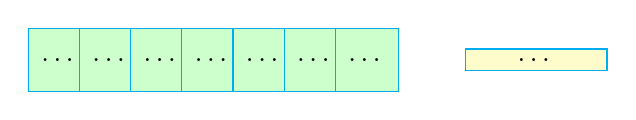
\begin{tikzpicture}
    \coordinate (s) at (0,0);
    \foreach \token in {\dots,\dots,\dots,\dots,\dots,\dots,\dots}{
      \node[fill=green!20, minimum size=8mm, draw=cyan, rectangle] at (s) {$\token$};
      \coordinate (s) at ($(s) + (0.65,0)$);
    }
    \coordinate (s) at ($(s) + (1.5,0)$);
    \node[fill=yellow!20, minimum width=18mm, draw=cyan, rectangle] at (s) {$\dots$};
  \end{tikzpicture}
  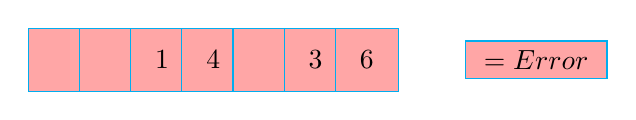
\begin{tikzpicture}
    \coordinate (s) at (0,0);
    \foreach \token in {\,,\,,1,4,\,,3, 6}{
      \node[fill=red!35, minimum size=8mm, draw=cyan, rectangle] at (s) {$\token$};
      \coordinate (s) at ($(s) + (0.65,0)$);
    }
    \coordinate (s) at ($(s) + (1.5,0)$);
    \node[fill=red!35, minimum width=18mm, draw=cyan, rectangle] at (s) {$=Error$};
	\end{tikzpicture}
	\\

  \captionof{mytype}{All Postfix Expressions for the Operand Permutation $[1,4,3,6]$}
  \label{all-ops-with-one-operand-arr}
  \end{arrangement}

An upper bound on all 7-token postfix expressions thus formed is: $64\times 840 = 53760$. We examine every expression and, if it is valid, check the result it produces. Some \emph{optimizations} can reduce the number of expressions we need to evaluate. We assume the availability\footnote{We implement them at [\ref{ss:impl}]} of procedures \texttt{\textcolor{teal}{perms, tuples, expr}}.  

Here is our algorithm [\ref{alg2}]:
\begin{algorithm}
\caption{An Algorithm to Solve Puzzle [\ref{puzzle1}]}
\label{alg2}
\begin{algorithmic}[2]
  \State $g \gets 24$ \Comment{Target result: 24}
  \State $f = false$  \Comment{Did we find an expression?}
  \State $P \gets \Call{perms}$ \Comment {$P\gets [P_1, P_2, \dots, P_{840}]$} 
  \State $T \gets \Call{tuples}$ \Comment {$T\gets [t_1, t_2, \dots, t_{64}]$} 
  \ForAll{$p \in P$}
    \ForAll{$t \in T$}
      \State $e \gets \Call {expr}{p, t}$ \Comment{$e\gets$ expression from given permutation and tuple}
      \State $r \gets \Call {evalPostFix}{e}$ \Comment{$r\gets$ the value using algorithm [\ref{alg1}]}
      \If{$r = g$}
        \Output {Bingo! Found a way to make g: $e$}
	\State $f = true$
      \EndIf
    \EndFor
  \EndFor
  \If {$f = false$}
        \State \Output {There's no way to make g!}
  \EndIf
\end{algorithmic}
\end{algorithm}
The algorithm [\ref{alg2}] is generic and therefore useful in practice.  Of course, many optimizations are possible. It is also extensible to unary operators like factorial. However, unary operators cause ambiguity because, unlike binary operators, they can be applied any number of times. For instance, if we use the unary $\sqrt{\phantom{x}}$ (square root) operator, the expression: $[16, \sqrt{\phantom{x}}, \sqrt{\phantom{x}}]$ makes 2 from 16.
\subsection{An Implementation}
\label{ss:impl}
A Java implementation of the algorithm [\ref{alg2}] is available at \cite{Fazlur}. It correctly produces the expressions that solve this and similar problems.
\section{Summary and Conclusion}

The author describes a surprising application of a technique he learned in grad school to solve a combinatorial puzzle he encountered on social media years later. Of course, there may be other techniques to solve the puzzle. 

The puzzle is simple enough for any curious layperson familiar with basic arithmetic to attempt and enjoy, but it begets some serious computational questions. 
\begin{enumerate}
\item Every possible expression must be examined. There is no ``shortcut'' to find the expression that evaluates to a target number. Must we examine every expression? Can we do \emph{better} than the mundane ``make and evaluate every expression'' method?

\item If someone claims to find an expression, however, we can efficiently verify if the claim is valid. 

\item For four operands, we have to analyze more than $50000$ expressions in the worst case. How many expressions might we have to analyze if the number of operands is 10? Or 20? 

\item If no expression evaluates to a given target, is there a trick that lets us \emph{quickly} conclude that without having to analyze every expression? In other words, do we have a more efficient algorithm to solve this puzzle in the negative case? 
\end{enumerate}

Here is another similar puzzle:
\begin{question}
\label{puzzle2}
How can you make $74$ using the numbers $1, 3, 4,$ and $6$ exactly once each, and the four arithmetic operations ($+, -, \times, \div$) any number of times\footnote{Using a number formed by concatenating two or more numbers (e.g. $13$) is not allowed}?

({\small Hint: The expression $((4\times6)+1)\times 3$ evaluates to 75.})

\end{question}

The puzzle represents one class of problems that pose challenges even to the fastest computers because an ``efficient'' algorithm may not exist\footnote{Try asking puzzle [\ref{puzzle2}] to an LLM like ChatGPT; you may not conclude that it is \emph{intelligent}}. Increasing the number of operands by an additive constant increases the number of cases to examine by a multiplicative constant. Who knows, if you can find an efficient algorithm for such problems or \emph{prove} that none exists, you may win a million dollars\footnote{See the \href{https://en.wikipedia.org/wiki/P_versus_NP_problem}{P versus NP Problem}}!

\section{Answer to the Original Puzzle}

Time for a handstand, maybe?

\begin{rotanswer}
$6\div(1-(3\div 4))$
\end{rotanswer}

%%%-----------------------------------------------------------------------------
\printbibliography % alternatively: \MakeBibliography[nosplit]
%%%-----------------------------------------------------------------------------

%%%-----------------------------------------------------------------------------
\end{document}
%%%-----------------------------------------------------------------------------

